\documentclass{tufte-handout}

\usepackage{../CommonLatexPackages/fall2018_preamble_v1.0}
\fancypagestyle{firstpage}

{\rhead{Day 2 \linebreak \textit{Version: \today}}}

\title{Day 2: Curves, Motion, and Neato}
\author{Quantitative Engineering Analysis}
\date{Spring 2019}

\begin{document}

\maketitle
\thispagestyle{firstpage}

\section{Schedule}
\bi
\item 0900-0920: Quiz
\item 0920-0940: Debrief
\item 0940-1030: Parametric Avenue
\item 1030-1045: Coffee
\item 1045-1215: Differential Drive in Action
\item 1215-1230: Preview of the Overnight
\ei

\section{Conceptual Quiz [20 minutes]}

\be
\item Match the following curves and vector functions

\begin{tabular}{ll}
1. $\r(u) = \cos u \ihat + \sin u \jhat$ & A. Helix \\
2. $\r(u) = \cos u \ihat + 2 \sin u \jhat$ & B. Circle \\
3. $\r(u) = (1+u) \ihat + (1+ 2u) \jhat$ & C. Ellipse \\
4. $\r(u) = \cos u \ihat + \sin u \jhat + 2u \khat$ & D. Straight-Line
\end{tabular}
\item A curve in 3D is described by the parametric function $\r(u)$. Which of the following statements are ALWAYS true (assuming the curve is smooth)?
\be
\item $\r'(u)$ is tangent to the curve.
\item $\r''(u)$ is normal to the curve.
\item $\Bhat = \khat$.
\item $\Nhat = \frac{\That'}{|\That'|}$.
\item The curvature $\kappa$  is constant.
\item The torsion $\tau$ is zero.
\item The length of the curve is $\int |\r'(u)|\; du$.
\ee
\item Two bodies move in 3D with position vector $\r_1(t)$ and $\r_2(t)$ respectively such that the curve they move along is identical, but the rate at which they move along it may be different. Which of the following statements are ALWAYS true (assuming that the motion is smooth)?
\be
\item At every point on the curve the velocity of body 1 is equal to the velocity of body 2 because they move along the same curve.
\item At every point on the curve the normal component of acceleration of body 1 is equal to the normal component of acceleration of body 2 because they move along the same curve.
\item At a given point on the curve, the normal component of acceleration of both bodies is equal if the two bodies have the same linear speed.
\item At a given point on the curve, the tangential acceleration of both bodies is equal if the two bodies move along the curve with different, but constant linear speeds.
\item Both bodies travel the same distance in the same amount of time.
\ee
\ee

\section{Debrief [20 minutes]}

Discuss the overnight with your table-mates, and make a list of concepts you feel solid on, and concepts you feel shaky on. Make a list of plus and deltas for this assignment. This debrief is short, but you will be applying the concepts from the overnight during the next exercise.

\section{The NEATO Goes for a Drive on Parametric Avenue [50 minutes]}
Here we will work to connect the work you did over the weekend to the upcoming challenge.

A hypothetical NEATO has just gone for a drive, and we have recorded its position vector $\r(t)$. Its path is shown below, and the dots indicate its position at equally-spaced points in time. It starts in the bottom left corner and moves along the path until it reaches the last point. Let's assume that this is a relatively long drive - the grid spacing is 1m and the time between samples is 1s. You can either work with this path, or you can draw your own curvy path on the board - just make sure you include discrete points and that the NEATO moves along the path you create in a non-uniform way. 

\newthought{You might want to use a NEATO sketched on a sticky note as a stand in for the NEATO as it moves along your path. If you prefer you could use your phone and try to make sense of the data from the sensors on the phone.}

\begin{figure}
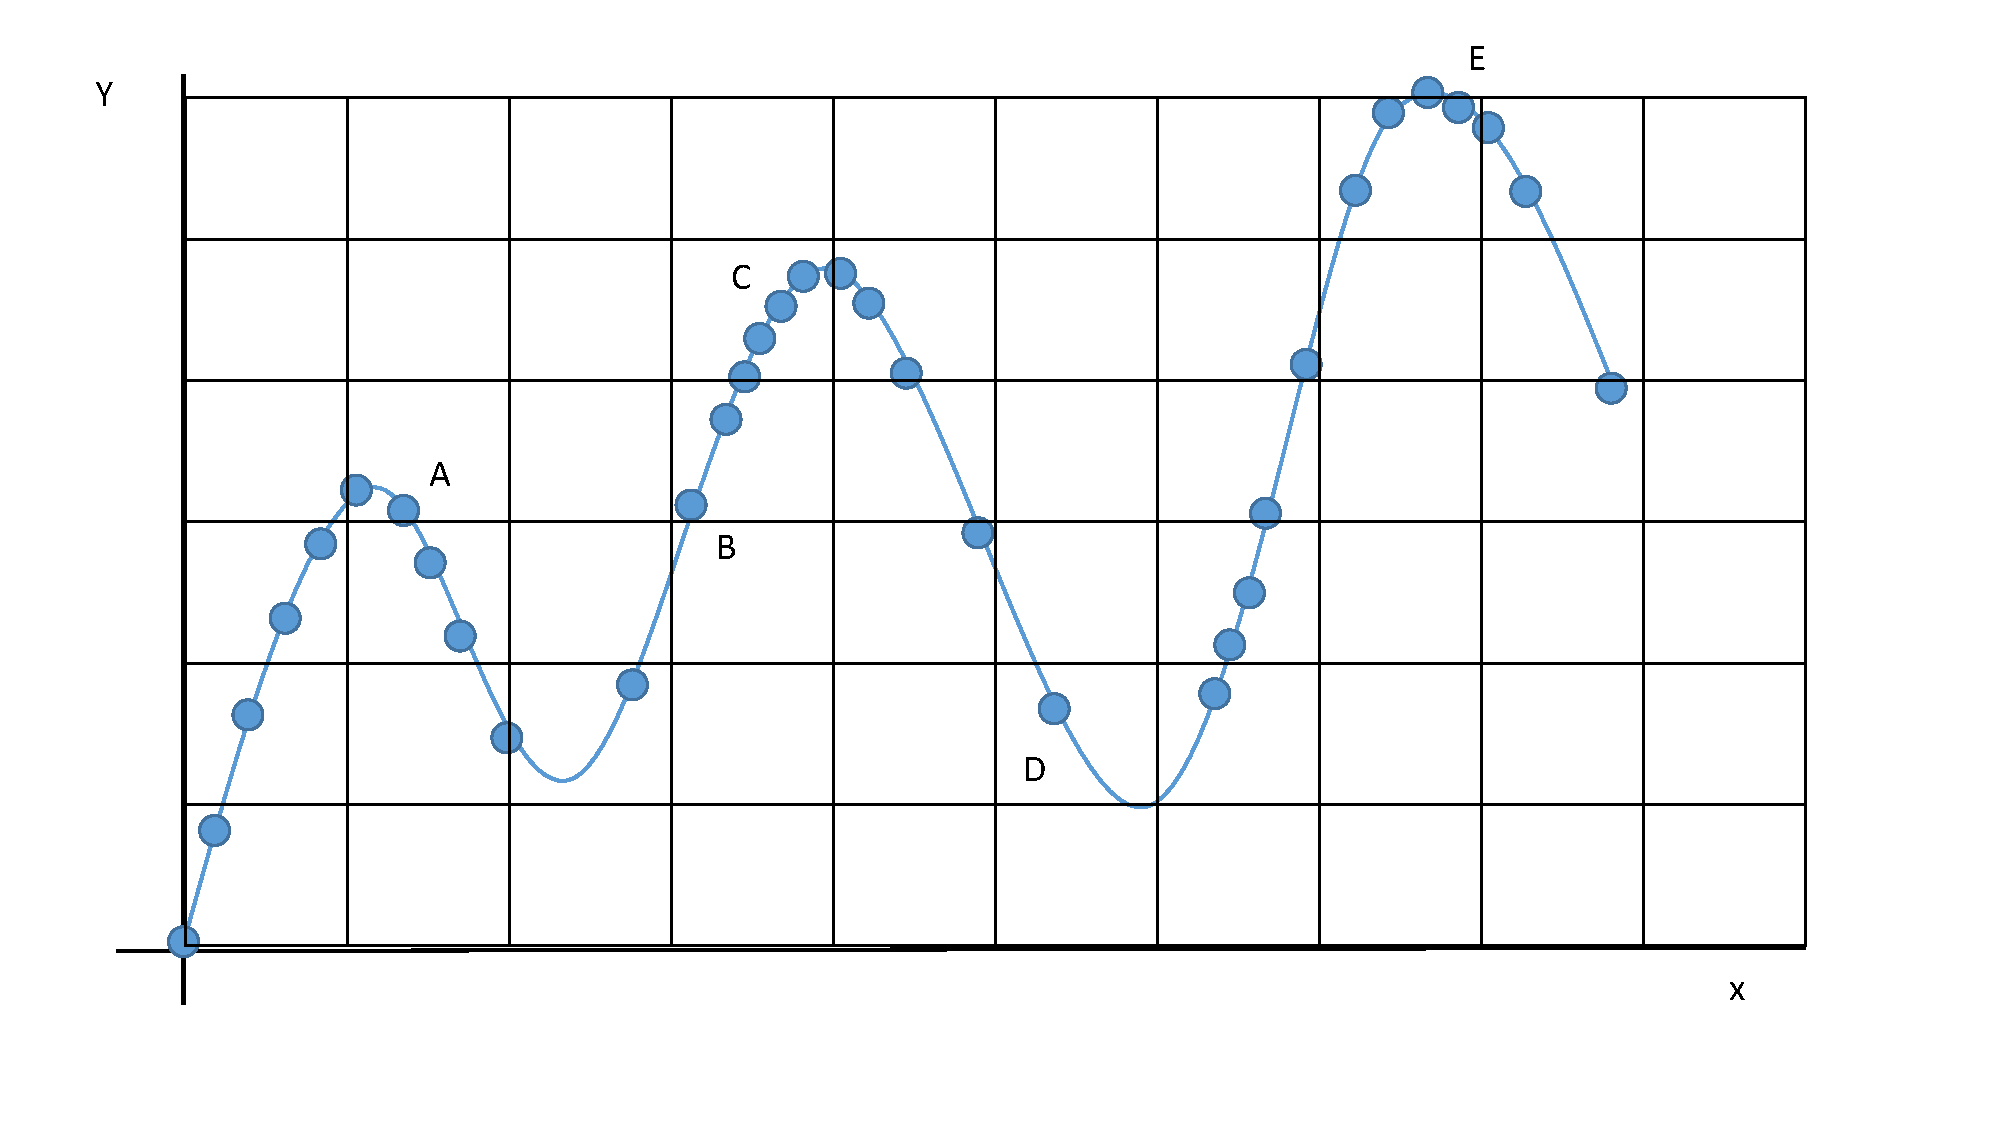
\includegraphics[width=5in]{figures/RandomCurve.pdf}
\end{figure}

\be
\item Roughly how long does the NEATO travel for? Roughly how far does it travel? Roughly what is its average speed? 
\item Thinking about the curve only, draw the unit tangent vector $\That$ and unit normal vector $\Nhat$ at each of the points indicated.
\item Thinking about the motion of the NEATO now, draw the velocity vector and acceleration vector at the same points. How do these relate to the unit tangent and unit normal vectors? What is their magnitude? Decompose the acceleration vector into tangential and normal components.
\item Draw a picture of the NEATO at A, B, C, D, and E, i.e. you are looking down on the NEATO as it drives along the curve.
\item  The NEATO has its own internally defined coordinate system which is fixed to the robot (this is called a 'body-fixed' coordinate system).  This coordinate system is used, among other things, for the readouts from the LIDAR scanner.  The NEATO's coordinate system has the $x$-axis pointing forward, the $y$-axis pointing left, and the $z$-axis pointing up.  For each of your NEATO pictures on the curve, indicate the orientation of the NEATO's own coordinate system.  How does this relate to the $\That$ and $\Nhat$ vectors?
\item  In order for the NEATO to follow the curve, what must be true about the orientation of the NEATO's $x$-axis as it traverses the curve? What about its $y$-axis?
\item  The NEATO is an example of a 'rigid body':  an object which has a size (unlike a point particle, which you often consider in introductory physics) but for which the different parts of the body do not move with respect to one another (no stretching, bending, etc).  When we study the motion of a rigid body, we can think about decomposing the motion into two components:  the motion OF the center of the object and the motion ABOUT the center of the object.  In other words, when we talk about the motion of the NEATO, in order to give a complete description, we need to specify the velocity of the center of the robot in the lab $x$ direction, the velocity of the center of the robot in the lab $y$ direction, and the rotational motion of the NEATO around its center. This system has three degrees of freedom:  $x$,$y$, and $\theta$ and we have to give the velocity for each!

\be

\item On your picture, indicate the orientation $\theta$ of the NEATO at each of the indicated points.  Define $\theta$ as the angle of the forward direction of the NEATO (NEATO's $x$ axis) measured counter-clockwise from the lab $x$ direction.

\item  The angular velocity $\boldsymbol \omega$ is a vector quantity whose magnitude gives the time rate of change of the orientation of the object and whose direction is the axis of rotation.  For an object constrained to move in 2 dimensions, we can express the angular velocity as
\[\boldsymbol \omega  = \omega \khat \]
where $\omega = d \theta / dt$ is the rate of change of angle of orientation. What direction is the angular velocity vector if the NEATO is curving to the right?  What direction is the angular velocity vector if the NEATO is curving to the left?  (Recall:  the angular velocity follows the right hand rule.  What characteristic vector of your parametric curve is also along this direction?

\item If the object is constrained to always be oriented along its path (a NEATO that isn't slipping for example), then a consistent mathematical definition of angular velocity $\boldsymbol \omega$  is
\[ \boldsymbol \omega  = \That \times \frac{d \That}{dt} \]
With this definition in mind, give a rough indication of the angular velocity of the NEATO at various points along the path. (This definition will be explored more in the overnight).  
\ee
    
\item Consider a NEATO that moves according to the following position vector
\[\r(t) = 0.05 t \ihat + 0.05 t^2 \jhat \]
where $\r(t)$ has units of meters and $t$ has units of seconds.

\be

\item On the board, sketch the path that the NEATO moves along in 10 seconds, roughly indicating its location every second.

\item Find the unit tangent vector and the unit normal vector.

\item Mathematically determine the linear velocity, the angular velocity, and the acceleration of the NEATO as it moves along the path.

\item Visualize the path and the unit vectors in MATLAB.
\ee

\ee

\section{Coffee [15 minutes]}

\section{Differential Drive in Action [90 minutes]}

In the first overnight you learned how to determine the velocity and acceleration of a particle moving along a parametric curve.  In the previous activity, you connected these quantities to the motion of the Neato moving along the curve.  Next, you'll extend this by considering not just the overall linear and rotational motion of the Neato as it moves along the curve, but how the motion of the Neato's wheels must be set in order to achieve this overall motion.  To accomplish this you'll be working through the basic mechanics of differential drive vehicles.  Specifically, you'll need to understand how the movement of each of the Neato's wheels translates into movement of the robot itself.  In this section you will be solving two important, and closely related, problems related to robot motion:
\begin{marginfigure}
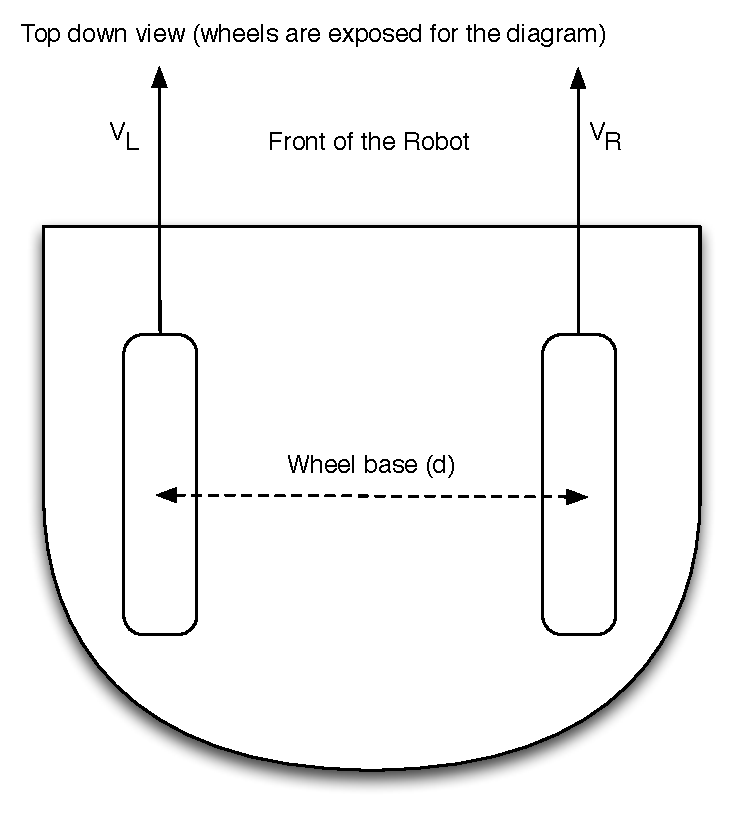
\includegraphics[width=6cm]{figures/differential_drive}
\caption{A diagram of the Neato's differential drive system.\label{fig:differential_drive}}
\end{marginfigure}

\begin{itemize}
\item [a.] Given a desired forward and angular velocity, determine the appropriate velocities of each of the robot's wheels.
\item [b.] Given the robot's current position, heading, and the velocities of its wheels, determine the robot's new position and heading.  \emph{Note: solving this problem can be quite useful when you have a sensor that estimates the actual wheel velocities of your robot (as the Neato does).  In this way you can correct for discrepancies between the intended motion and what your robot actually did.}
\end{itemize}

%Thinking back to day 1 in class, these problems are analogous to the forward and inverse kinematics problems we solved for robotic manipulators.  The key difference is that in day 1 we were interested in how degrees of freedom in the configuration space (e.g., joint angles of the robotic manipulator) translated into the position of the robot in the world.  Here, we are interested in how degrees of freedom in phase space (which includes velocities in addition to positions) translate into velocities of the robot in the world.

\paragraph{Formalizing the Problem}
The Neato has two wheels equally spaced about its centerline (see Figure~\ref{fig:differential_drive}).  As we saw during day 1, driving the wheels at different velocities (labeled $V_L$ and $V_R$ in the diagram) will achieve different linear and angular velocities.%  This drive mechanism is called differential drive, and it is one of the most common for ground robots.

\begin{myboxi}[Exercise 1]
In day 1 of this module you built up an intuition for how movement of each of the wheels for a differential drive vehicle would translate into motions of the robot.  Before we dive into a quantitative treatment of the subject, let's remind ourselves of some limiting cases.  Determine qualitatively how the Neato would move (in terms of both linear and rotational motion) in these cases.
\begin{itemize}
\item What if both wheels move forward (positive velocity) with equal speed?
\item What if both wheels move backward (negative velocity) with equal speed?
\item What if one wheel drives forward and the other moves backward with equal speed?
\item What if one wheel drives forward while the other remains stationary?
\end{itemize}
For each limiting case draw some key frames depicting your prediction of the robot's behavior over several instants in time.
\end{myboxi}

Now that you have refreshed your intuition, let's solve the problem quantitatively.  The key insight is that the robot cannot move laterally, but instead must have a linear velocity parallel to the direction of its wheels. As the robot moves along a curve, the robot rotates about its center in order to keep itself aligned with the forward motion. Let's assume that the center of rotation of the robot is located midway between the wheels.

\vspace{1em}
\begin{myboxi}[Exercise 2]
Assuming no wheel slippage, the linear velocity $V$ and angular velocity $\omega$ can be expressed in terms of the left and right wheel velocities $V_L$ and $V_R$, and the robot's wheel base $d$ (the distance between the two wheels).
\begin{align}
V &= \frac{V_L + V_R}{2} \\
\omega &= \frac{V_R - V_L}{d}
\end{align}
Does this make sense? Can you confirm these expressions? Can you think of some test cases to validate these expressions? (hint: you just thought about some in the previous exercise!)
\end{myboxi}
\vspace{1em}

\vspace{1em}
\begin{myboxi}[Exercise 3]
Solve equations (1) and (2) in order to express the left and right wheel velocities in terms of the linear and angular velocities and wheel base and show that
\begin{align}
V_L &= V - \omega \frac{d}{2} \\
V_R &= V + \omega  \frac{d}{2}
\end{align}
Does this make sense? Can you think of some test cases to validate these expressions?
\end{myboxi}
\vspace{1em}


\subsection{Validating your Model}\label{sec:validating_your_model}
The equations in the previous section define a motion model for your robot.  As with any model, you shouldn't expect it to be perfect.  Next, you will be designing and carrying out an experiment to determine the strengths and weaknesses of your model.
\vspace{1em}
\begin{myboxi}[Exercise 4]
There are many ways to validate the motion model of your robot.  Design a few experiments that one could perform in order to establish the accuracy of your model.  This question is meant to help you think conceptually about what it means to do validation in this context, so \textbf{don't get hung up designing an experiment that you will actually be performing (that is the point of the \emph{next} question)}.  For each experiment, specify the following.
\begin{enumerate}
\item What is the goal of your experiment (i.e., what are you trying to validate)?  Some experiments will be appropriate for validating that your model has the right qualitative behavior.  These sorts of experiments are useful for catching discrepancies between the model you tried to work out and the equations you actually derived.  Other experiments are useful for validating your model quantitatively.  For instance, you might be interested in determining the accuracy of your model, or determining an optimal value for some model parameter.
\item Describe the experimental procedure.  What motor commands will you send to the robot (e.g., you will send commands to have the robot drive straight for 10 seconds)?
\item What will you observe and/or measure?
\item How will the observations or measurements help you achieve the goals enumerated in (1)?
\item Are there any weaknesses in your proposed experiment?  Another way to think about it is: are there any major assumptions you have to make in order to carry out the experiment?  \textbf{Every method of validation has weaknesses, this question is designed to prompt you to think about and then articulate these explicitly.}
\end{enumerate}
It may help to think about some equipment for measuring robot motion.  What if you used the motion capture lab?  What if you validated your model outside with your phone's GPS?  What if you only had access to a ruler and a protractor?
\end{myboxi}
\vspace{1em}

\begin{myboxi}[Exercise 5: actually using the NEATO. Yay!]
Choose an experiment (or family of experiments) to perform to validate the accuracy of the motion model of your robot.  Your experiment should be something that is relatively easy to do (i.e. uses simple tools) and has a well-defined and easy to compute measure of your model's error with respect to the collected data.  We suggest choosing fixed values for $V_L$ and $V_R$ using a command of the form (where V\_L and V\_R are the left and right wheel velocities that should be updated):

\begin{verbatim}
pub = rospublisher('/raw_vel');
msg = rosmessage(pub);
msg.Data = [V_R, V_L];
send(pub, msg);

prompt = 'Press Enter to Stop Robot';
str = input(prompt,'s');
if isempty(str)
    msg.Data=[0,0];
    send(pub,msg)
end
\end{verbatim}

In this example block of code you will use the \emph{input} function to wait until the user presses \emph{enter} before stopping the robot. In the overnight you will explore using the \emph{tic} and \emph{toc} functions to have the robot drive for a set period of time. 

For your estimated value of $d$ (which you can obtain by directly measuring the wheel base), determine the predicted motion of your robot.  Make a table of this prediction versus your robot's actual behavior for at least 3 trials.  Hint: if you chose to use fixed values of $V_L$ and $V_R$ you may consider comparing the predicted total rotation and/or the predicted radius of curvature of your robot to your measurements of these quantities.  Compute the total error between your predictions and the measurements of the robot's behavior.  Compare the accuracy of your predictions for slightly different values of $d$ (both higher and lower) with those for the measured value of $d$.  Which value of $d$ appears to be best?  Do you have any theories as to the sources of error that could be causing your model not to be 100\% accurate?


If you have time, you can also try comparing your results to using the \emph{/cmd\_vel} Ros topic which takes data in the form of a \emph{twist} message which takes the \textbf{linear} and \textbf{angular} velocities instead of the left and right wheel velocities. Try running the code below (replace V\_linear and V\_angular) and compare the results to the experiments you performed using $V_L$ and $V_R$.

\begin{verbatim}pub = rospublisher('/cmd_vel');
msg = rosmessage(pub);
msg.Linear.X = V_linear;
msg.Angular.Z = V_angular;
send(pub, msg);

prompt = 'Press Enter to Stop Robot';
str = input(prompt,'s');
if isempty(str)
    msg.Linear.X = 0;
    msg.Angular.Z = 0;
    send(pub,msg)
end
\end{verbatim}


\end{myboxi}

%\section{Derivation (optional)}
%Suppose we have a parametric curve $\mathbf{r}(t) = f(t) \hat{\mathbf{i}} + g(t) \hat{\mathbf{j}}$.  We saw in the overnight that the tangent vector is given by $\mathbf{T}(t) = f'(t) \hat{\mathbf{i}} + g'(t) \hat{\mathbf{j}}$.  Further, if the robot moves along the path, tangent to the curve, its forward speed will be $\|\mathbf{T}(t)\|$.
%%
%%\begin{marginfigure}
%%\begin{center}
%%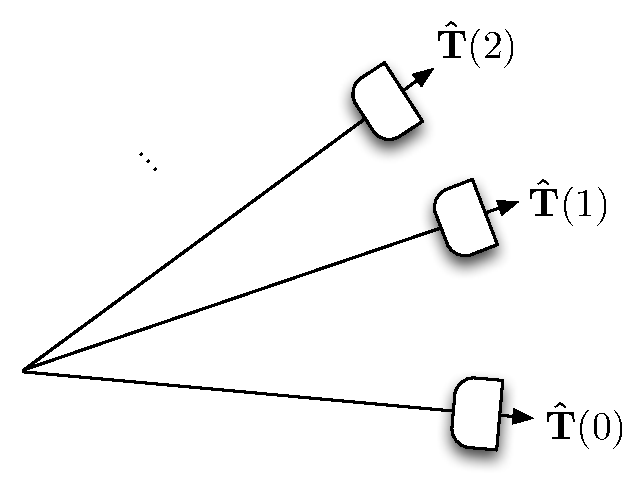
\includegraphics[width=\linewidth]{figures/angular_velocity_derivation}
%%\end{center}
%%\caption{The change in the robot's heading over time.  The shapes at the end of the arrows are supposed to depict the robot (with the flat side being straightahead).  Since $\hat{\mathbf{T}}$ is a unit vector the robot will move about the unit circle.\label{fig:angularvel}}
%%\end{marginfigure}
%
%Determining expression you have been using for the angular velocity $\omega(t)$ of our robot is more involved.  Before we derive the correct expression, we will introduce the notion of angular velocity vectors, which you may or may not have seen before.  While expressing angular velocity as a vector may at first seem overly complex (since in this case we know that the robot will rotate about the z-axis, and it seems like we should just be able to compute the scalar magnitude along with whether to turn clockwise or counterclockwise), thinking about the angular velocity as a vector will enable our derivation to be done in a much more straightforward and generalizable manner.
%
%Angular velocity vectors point in the direction about which the body rotates (which for our robot will be along either the positive or negative z-axis).  For right-handed coordinate systems (such as the one we are using here), by convention the rotation happens counterclockwise about the direction of the rotation axis.  Further, the magnitude of the vector indicates the angular speed.
%
%In the problem at the beginning of class on Monday we discussed the coordinate system attached to the robot:  the body fixed frame.  Because the heading of the robot is locked to the tangent vector $\hat{\mathbf{T}}$ of the curve, we can think of the vector $\hat{\mathbf{T}}$ as being a constant in the body fixed frame of the robot.  The body fixed frame is rotating with some unknown angular velocity vector \textbf{$\Omega$} with respect to the room coordinate system.  If we wish to know the time derivative of the tangent vector $\hat{\mathbf{T}}(t)$ in the room coordinate system, we can use the generalized relationship between the time derivatives of vectors in two coordinate systems which are rotating with an angular velocity vector \textbf{$\Omega$} with respect to each other.  This expression is
%\begin{equation}
%\frac{d\hat{\mathbf{T}}}{dt}|_{lab} = \frac{d\hat{\mathbf{T}}}{dt}|_{body} + \textbf{$\Omega$} \times \hat{\mathbf{T}}
%\end{equation}
%
%(Full mathematical derivation \href{http://envsci.rutgers.edu/~broccoli/dynamics_lectures/lect_06_dyn12_mom_eq_rot.pdf}{here} , nice heuristic explanation \href{https://ocw.mit.edu/courses/aeronautics-and-astronautics/16-07-dynamics-fall-2009/lecture-notes/MIT16_07F09_Lec08.pdf}{here}) In the body frame of the robot, $\hat{\mathbf{T}}$ is unchanging, since it is always aligned with the forward direction, so the term $\frac{d\hat{\mathbf{T}}}{dt}|_{body}$ is zero leaving us with
%\begin{equation}
%\frac{d\hat{\mathbf{T}}}{dt}|_{lab} = \textbf{$\Omega$} \times \hat{\mathbf{T}}
%\end{equation}
%
%%To compute the angular velocity vector we can start from the relationship between rotational and angular velocities.
%%\begin{align}
%%\mathbf{v}(t) &= \mathbf{\omega}(t) \times \mathbf{r}(t) \nonumber
%%\end{align}
%
%%If we substitute in $\hat{\mathbf{T}}(t)$ for $\mathbf{r}(t)$ and
%
%Then we make use of the \href{https://en.wikipedia.org/wiki/Triple_product}{scalar triple product}, which states that $\mathbf{a}\times (\mathbf{b}\times \mathbf{c}) = \mathbf{b}(\mathbf{a}\cdot\mathbf{c}) - \mathbf{c}(\mathbf{a}\cdot\mathbf{b}$).  Using this we can derive our angular velocity vector.
%
%%Note: that $\mathbf{v(t)}$ in this case is the derivative of $\hat{\mathbf{T}}(t)$ which is $\mathbf{N}(t)$.
%
%\begin{align}
%\frac{d\hat{\mathbf{T}}(t)}{dt}|_{lab} &= \textbf{$\Omega$}(t) \times \mathbf{\hat{T}}(t) \nonumber \\
%\mathbf{N}(t) &= \textbf{$\Omega$}(t) \times \mathbf{\hat{T}}(t) \nonumber \\
%\mathbf{\hat{T}}(t) \times \mathbf{N}(t) &= \mathbf{\hat{T}}(t) \times \textbf{$\Omega$}(t) \times \mathbf{\hat{T}}(t) \nonumber \\
%&= \textbf{$\Omega$}(t) (\hat{\mathbf{T}}(t) \cdot \hat{\mathbf{T}}(t) ) - \hat{\mathbf{T}}(t) (\hat{\mathbf{T}}(t) \cdot \mathbf{w}(t)) \nonumber \\
%&= \textbf{$\Omega$}(t) (1) - \hat{\mathbf{T}}(t) (0) \nonumber \\
%&=  \textbf{$\Omega$}(t) \nonumber \\
%\textbf{$\Omega$}(t) &= \mathbf{\hat{T}}(t) \times \mathbf{N}(t)
%\end{align}
%The x and y components of the angular velocity vector will always be 0.  The magnitude of the z-component is the angular speed.  If the z-component is positive, we turn counterclockwise at that speed.  When it is negative, we should turn clockwise at that speed.


\end{document}
